\documentclass[11pt]{article}

\input{../../utils/preamble_problemas}

\title{Introducción a la física}
\author{Manuel Carlevaro}
\date{Universidad de Navarra}


\begin{document}
%\maketitle

\begin{center}
\framebox[1.0\textwidth][c]{
\huge{\textsc{Introducción a la física}} 
}
\end{center} 

\begin{center}
\vspace{1em}
\Large{\textsc{Universidad de Navarra}} 
\end{center}

 \vspace{1em}

\begin{center}
\begin{tabular}{r l}
 \textbf{Tema:} & Vectores.\\
 \textbf{Profesor:} & Manuel Carlevaro \\
\end{tabular}\end{center}

\vspace{2em}

\begin{exercise}
\begin{multicols}{2}
\begin{center}
    \includegraphics[scale=0.35]{figs/ruta.png}
\end{center}
\begin{enumerate}[a)]
    \item Una persona conduce su coche por la ruta de la figura. Determine la magnitud y la dirección del desplazamiento resultante dibujando un diagrama a escala (la figura no está a escala).
    \item Utilice el método de las componentes para hallar la resultante de los desplazamientos de la parte a).
\end{enumerate}
\end{multicols}
\end{exercise}

\begin{exercise}
    \begin{multicols}{2}
        \begin{center}
            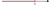
\includegraphics[scale=0.85]{figs/fig-08.pdf}
        \end{center}

        Dados los vectores de la figura, halle:
        \begin{enumerate}[a)]
            \item Las componentes de cada vector.
            \item Las sumas y restas $\vect{a} + \vect{b}$, $\vect{b} + \vect{a}$, $\vect{a} - \vect{b}$, $\vect{b} - \vect{a}$. 
            \item Los productos escalares $\vect{a} \cdot \vect{b}$, $\vect{b} \cdot \vect{c}$ y $\vect{a} \cdot \vect{c}$. 
            \item Los productos vectoriales $\vect{a} \mul \vect{d}$ y $\vect{d} \mul \vect{a}$.
        \end{enumerate}
    \end{multicols}
\end{exercise}

\begin{exercise}
    Calcule el ángulo entre los vectores $\vect{a} = -2 \hat{\bm{i}} + 6 \hat{\bm{j}}$ y  $\vect{b} = 2 \hat{\bm{i}} - 3 \hat{\bm{j}}$.
\end{exercise}

\begin{exercise}
    Resuelva el ejercicio anterior agregando la tercera dimensión (con componentes nulas) y usando el producto vectorial.
\end{exercise}

\begin{exercise}
    \begin{multicols}{2}
        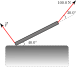
\includegraphics[scale=0.90]{figs/fig-09.pdf}

        Decimos que un objeto está en equilibrio cuando todas las fuerzas sobre él se estabilizan (suman cero). La figura muestra una viga que pesa \qty{124}{N} y que está apoyada en equilibrio por una fuerza de \qty{100}{N} y una fuerza $\vect{F}$ en el piso. La tercera fuerza sobre la viga es el peso de \qty{124}{N} que actúa verticalmente hacia abajo.
        \begin{enumerate}[a)]
            \item Utilice componentes de vectores para encontrar la magnitud y la dirección de $\vect{F}$.
            \item Verifique lo razonable de su respuesta en el inciso a) haciendo una solución gráfica aproximadamente a escala.
        \end{enumerate}
    \end{multicols}
\end{exercise}

\begin{exercise}
    En la molécula de metano, CH$_4$, cada átomo de hidrógeno está en la esquina de un tetraedro regular, con el átomo de carbono en el centro. En coordenadas en las que uno de los enlaces C--H esté en la dirección $\hat{\bm{i}} + \hat{\bm{j}} +\hat{\bm{k}}$, un enlace C--H adyacente está en la dirección  $\hat{\bm{i}} - \hat{\bm{j}} -\hat{\bm{k}}$. Calcule el ángulo entre dos enlaces.
\end{exercise}

\end{document}
